\begin{activity} \label{PA:10.13} 
\ba
\item Figure \ref{F:10.5.tree.2} shows the tree diagram we construct when (a) $z$ depends on $w$, $x$, and $y$, (b) $w$, $x$, and $y$ each depend on $u$ and $v$, and (c) $u$ and $v$ depend on $t$.

\begin{figure}[ht]
  \begin{center}
    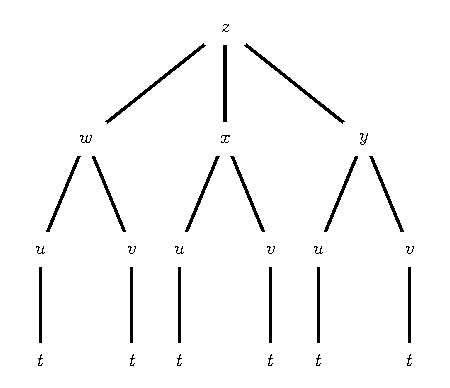
\includegraphics{figures/fig_10_5_tree_2.eps}
  \end{center}
  \caption{Three levels of dependencies}
  \label{F:10.5.tree.2}
\end{figure}

\begin{enumerate}[i.]
  \item Label the edges with the appropriate derivatives.
  \item Use the Chain Rule to write $\ds\frac{dz}{dt}$.
\end{enumerate}

\item Suppose that $z=x^2 - 2xy^2$ and that 
    \begin{align*}
      x&=r\cos\theta \\
      y&=r\sin\theta.
    \end{align*}
    \begin{enumerate}[i.]
	\item Construct a tree diagram representing the dependencies of $z$ on $x$ and $y$ and $x$ and $y$ on $r$ and $\theta$. 
	\item Use the tree diagram to find $\frac{\partial z}{\partial r}$. 
	\item Now suppose that $r = 3$ and $\theta=\pi/6$. Find the values of $x$ and $y$ that correspond to these given values of $r$ and $\theta$, and then use the Chain Rule to find the value of the partial derivative $\frac{\partial z}{\partial \theta}|_{(3,\frac{\pi}{6})}$.
    \end{enumerate}
    
  \ea

\end{activity} 

\begin{activitySolution}
\ba
\item 
	\begin{enumerate}[i.]
	\item A labeled tree diagram is shown here.
\begin{center}
\setlength{\unitlength}{1.5cm}
\begin{picture}(5,3.1)
\put(2,3){$z$}
\put(0.5,2){$w$}
\put(2,2){$x$}
\put(3.5,2){$y$}
\put(0,1){$u$}
\put(1,1){$v$}
\put(1.5,1){$u$}
\put(2.5,1){$v$}
\put(3,1){$u$}
\put(4,1){$v$}
\put(0,0){$t$}
\put(1,0){$t$}
\put(1.5,0){$t$}
\put(2.5,0){$t$}
\put(3,0){$t$}
\put(4,0){$t$}
\put(0.05,0.25){\line(0,1){0.65}}
\put(1.05,0.25){\line(0,1){0.65}}
\put(1.55,0.25){\line(0,1){0.65}}
\put(2.55,0.25){\line(0,1){0.65}}
\put(3.05,0.25){\line(0,1){0.65}}
\put(4.05,0.25){\line(0,1){0.65}}
\put(0.1,1.2){\line(3,5){0.4}}
\put(1,1.2){\line(-3,5){0.4}}
\put(1.6,1.2){\line(3,5){0.4}}
\put(2.5,1.2){\line(-3,5){0.4}}
\put(3.1,1.2){\line(3,5){0.4}}
\put(4,1.2){\line(-3,5){0.4}}
\put(0.75,2.25){\line(3,2){1}}
\put(2.075,2.25){\line(0,1){0.65}}
\put(3.25,2.25){\line(-3,2){1}}
\put(-0.25,0.5){$\frac{du}{dt}$}
\put(0.75,0.5){$\frac{dv}{dt}$}
\put(1.25,0.5){$\frac{du}{dt}$}
\put(2.25,0.5){$\frac{dv}{dt}$}
\put(2.75,0.5){$\frac{du}{dt}$}
\put(3.75,0.5){$\frac{dv}{dt}$}
\put(-0.1,1.5){$\frac{\partial w}{\partial u}$}
\put(0.9,1.5){$\frac{\partial w}{\partial v}$}
\put(1.4,1.5){$\frac{\partial x}{\partial u}$}
\put(2.4,1.5){$\frac{\partial x}{\partial v}$}
\put(2.9,1.5){$\frac{\partial y}{\partial u}$}
\put(3.9,1.5){$\frac{\partial y}{\partial v}$}
\put(0.85,2.65){$\frac{\partial z}{\partial w}$}
\put(1.75,2.5){$\frac{\partial z}{\partial x}$}
\put(2.85,2.65){$\frac{\partial z}{\partial y}$}
\end{picture}
\end{center}

	\item According to the Chain Rule we have 
\[\frac{dz}{dt} = \frac{\partial z}{\partial w}\frac{\partial w}{\partial u}\frac{du}{dt} + \frac{\partial z}{\partial w}\frac{\partial w}{\partial v}\frac{dv}{dt} + \frac{\partial z}{\partial x}\frac{\partial x}{\partial u}\frac{du}{dt} + \frac{\partial z}{\partial x}\frac{\partial x}{\partial v}\frac{dv}{dt} + \frac{\partial z}{\partial y}\frac{\partial y}{\partial u}\frac{du}{dt} + \frac{\partial z}{\partial y}\frac{\partial y}{\partial v}\frac{dv}{dt}.\]
	\end{enumerate}
\item 
	\begin{enumerate}[i.]
	\item A tree diagram is shown here.
\begin{center}
\setlength{\unitlength}{1.0cm}
\begin{picture}(2.5,3.5)
\put(-0.9,0.5){$r$} %Under x
\put(-0.65,0.85){\line(2,3){0.6}}
\put(0.7,0.5){$\theta$}
\put(0.65,0.85){\line(-2,3){0.6}}
\put(1.1,0.5){$r$} %Under y
\put(1.35,0.85){\line(2,3){0.6}}
\put(2.7,0.5){$\theta$}
\put(2.65,0.85){\line(-2,3){0.6}}
\put(0,2){$x$}
\put(-0.85,1.3){$\frac{\partial x}{\partial r}$}
\put(2,2){$y$}
\put(2.45,1.3){$\frac{\partial y}{\partial \theta}$}
\put(0.5,1.3){$\frac{\partial x}{\partial \theta}$}
\put(1.2,1.3){$\frac{\partial y}{\partial r}$}
\put(1,3.5){$z$}
\put(0.25,2.35){\line(2,3){0.6}}
\put(0.0,2.9){$\frac{\partial z}{\partial x}$}
\put(1.75,2.35){\line(-2,3){0.6}}
\put(1.6,2.9){$\frac{\partial z}{\partial y}$}
\end{picture}
\end{center}
	\item By the Chain Rule we have 
\[\frac{\partial z}{\partial r} = \frac{\partial z}{\partial x}\frac{\partial x}{\partial r} + \frac{\partial z}{\partial y}\frac{\partial y}{\partial r}.\]
	\item First note that $x(3,\pi/6) = 3\frac{\sqrt{3}}{2}$ and $y(3,\pi/6) = \frac{3}{2}$. Given that $z_x = 2x-2y^2$ and $z_y = -4xy$ we have $z_x(3, \pi/6)=3\sqrt{3}-3$ and $z_y(3,\pi/6) = -9\sqrt{3}$. Also, $x_r=\cos(\theta)$ and $y_r = \sin(\theta)$, so $x_r(3,\pi/6) = \frac{\sqrt{3}}{2}$ and $y_r(3,\pi/6) = \frac{1}{2}$. So  
\[\frac{\partial z}{\partial \theta}\bigm|_{(3,\frac{\pi}{6})} = (3\sqrt{3}-3)\left(\frac{\sqrt{3}}{2}\right) - 9\sqrt{3}\left(\frac{1}{2}\right).\]
	
	\end{enumerate}

\ea
\end{activitySolution}

\afterpa 
